\section{Methods and results}
With the implementation of the PML and using the algorithm \ref{algo}, we can now proceed to the test of the one dimensional PML. To evaluate the performance, we will focus on the reflection of the wave from the interface and the wave coming back from the PML. The other parameter to be evaluate will be the computational cost in term of time. In fact the objective of such analysis is to find the best compromise between accuracy, minimising the reflection wave and the computational. Therefore we will be able to highlight the parameters to have the best result possible.
\subsection{Inputs and parameters}
In order to test the PML, we choose to place ourselves in the context of the problem described by the figure \ref{fig:sch_pml}. A summary of the parameters used for the simulation can be found in the following table.
\begin{table}[H]
    \centering
    \begin{tabular}{c|c}
         $L_m$ & 50  \\
         $L_p$ & 20 \\
         $L_e$ & 1 \\
         $S$ & 1 \\
         $c_s$ & 50 \\
         $\rho$ & 1700\\
         E & $10e^5$ \\
         h & $0.8 h_{CFL}$ \\
         T & $500$ \\
    \end{tabular}
    \caption{Parameters for the PML and the medium}
    \label{tab:param}
\end{table}
In the table \ref{tab:param}, $T$ stands for the end time. The time step $h$ must be chosen carefully. This parameter is very important since we seek a balance between computational cost and accuracy. Of course increasing this parameter leads to a lower computational cost but also to a smaller accuracy. Another property determined by this parameter is also the stability of the numerical scheme. The method implemented in our case uses a GC coupled interface in order to be able to perform an explicit scheme on the medium while conserving an implicit one on the PML. Since explicit Newmark scheme is conditionally stable we need to ensure that the time step is smaller than the critical time step determine by the formula:
\begin{equation}
    h_{CFL} = \frac{L_e}{\sqrt{\frac{E}{\rho}}}
\end{equation}
A simple numerical application gives us in our case $h_{CFL} = 0.0412$. We ensured that the time step is below this critical time step.
The parameters for the Newmark-$\beta$ scheme are $\gamma=0.5$ and $\beta=0.25$.
The last parameters to define are the ones for the attenuation functions. The order of the polynomials will be $m=2$. The coefficients for the attenuation function for propagating wave is the most important to define due to its importance for the damping of the wave. If we assume that $\frac{c_s}{L_p}=1$, the coefficient for this function and in the case of a propagating P-wave in a one dimensional medium can be expressed by the following formula \cite{Kucukcoban2}:
\begin{equation}
    \alpha_p = \frac{(m+1)v_p}{2 L_{p}}log\left( \frac{1}{R} \right)
\end{equation}
where $v_p$ is the velocity of the P-waves and $R$ is the reflection coefficient from the outer PML boundary. This coefficient shows the amplitude reduction of the P wave entering into the PML. This parameter has to be taken into account when we will evaluate the performance of the method. The value for the parameters in the expression of the coefficient $\alpha_p$ has, in our example, the following values:
\begin{table}[H]
    \centering
    \begin{tabular}{c|c}
         $v_p$ & $76.7$  \\
         $R$ & $10^{-3}$ \\
         $\alpha_e$ & 1 
    \end{tabular}
    \caption{Parameters for the attenuation functions}
    \label{tab:param_attenuations}
\end{table}
As shown in the table \ref{tab:param_attenuations}, the coefficient of attenuation for evanescent wave is simply $0$. Since this function does not have a large impact on the damping of the wave entering the PML: $f^e(x)=0 \forall x$. 

\subsection{Ricker wave}
In this numerical simulation, we will analyse the behavior of the PML against the propagation of non harmonic waves. A Ricker wave will be imposed at the free end of the physical medium in the form of a force. This external force has the following formula:
\begin{equation}
    F_{ext} = A\left( 2 \pi^2\frac{(t-t_s)^2}{t^2_p}-1\right) exp\left( -\pi^2\frac{(t-t_s)^2}{t^2_p}\right)
\end{equation}
The Ricker wave is defined by 3 parameters: The fundamental period $t_p$, the time shift $t_s$ and the amplitude $A$. These parameters take the values:
\begin{table}[H]
    \centering
    \begin{tabular}{c|c}
         $t_p$ & 0.5s \\
         $t_s $& 1s \\
         $A$ & 1
    \end{tabular}
    \caption{Values for the parameters of the Ricker Wave}
    \label{tab:param_Ricker}
\end{table}
Using this parameters the Ricker wave in the time domain has the following shape:
\begin{figure}[H]
    \centering
    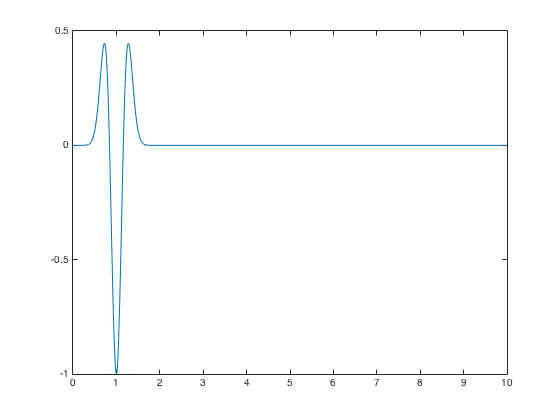
\includegraphics[scale=0.5]{images/ricker.png}
    \caption{Ricker wave in the time domain}
    \label{fig:ricker}
\end{figure}
\subsection{Results}
The measurement of the displacement and the velocity at the center of the physical medium gives a good insight of the propagation of the wave and of its possible reflection. Using the above parameters for the medium, the PML and the input wave, the following graphs are obtained:
\begin{figure}[H]
\centering
\begin{minipage}{.5\textwidth}
  \centering
  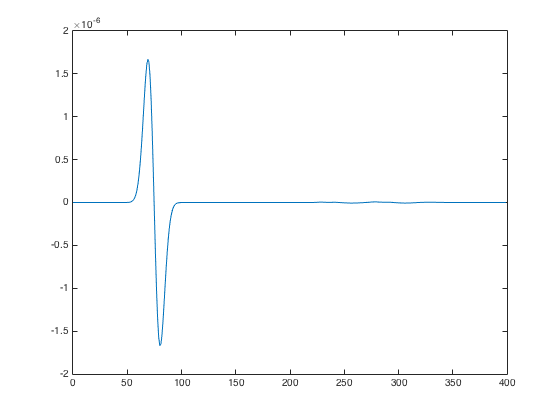
\includegraphics[width=.9\linewidth]{images/disp_med.png}
\end{minipage}%
\begin{minipage}{.5\textwidth}
  \centering
  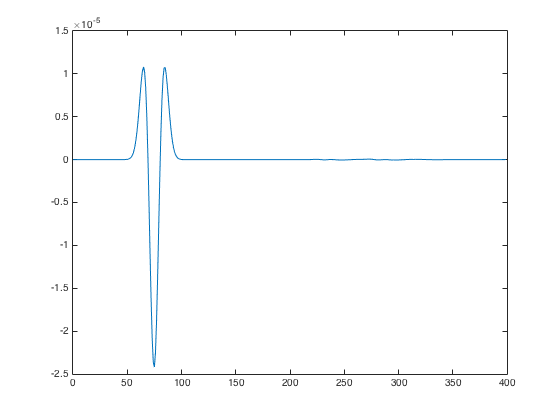
\includegraphics[width=.9\linewidth]{images/vel_med.png}
\end{minipage}
\caption{Longitudinal displacement (right) and the velocity (left) at $x=25m$ as a function of time}
\label{fig:disp_vel_improved}
\end{figure}

The figure \ref{fig:disp_vel_improved} shows the displacement and the velocity through the time at the node placed at $x=25m$. 
Looking at the figures \ref{fig:disp_vel_improved} we can see that the PML reduced drastically the reflection of the incident wave at the interface. Therefore the PML seems accurate since we can barely see the reflection of the wave at the interface. \\

\subsubsection{Reflection of the wave}
In this part, we will focus on the reflection of the wave in function of different parameters. To be more precise, we will separate the reflection of the wake into two kinds: the reflection due to the interface and the reflected wave bouncing at the extremity of the PML and coming back into the medium. This study will focus on the effect of the parameters for the PML such as the length $L_p$ and the attenuation coefficient $\alpha_p$. The length of the elements $L_e$ will also be tested and the last parameter tested will be the time step $k$.\\ 
First of all let us focus on the effect of the attenuation coefficient $\alpha_p$.
\begin{figure}[H]
\centering
\begin{minipage}{.5\textwidth}
  \centering
  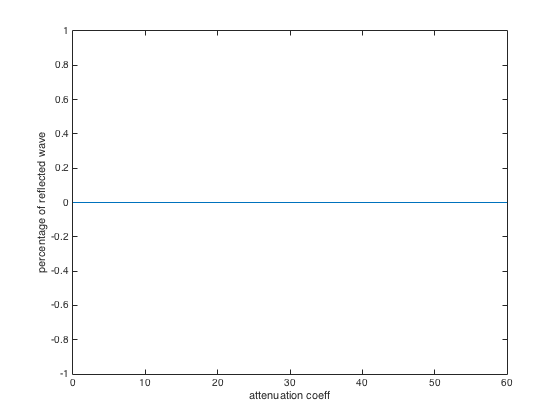
\includegraphics[width=.8\linewidth]{images/reflected_alphap.png}
\end{minipage}%
\begin{minipage}{.5\textwidth}
  \centering
  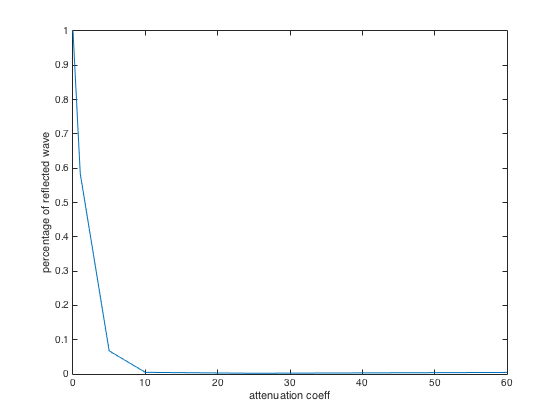
\includegraphics[width=.8\linewidth]{images/bouncing_alphap.png}
\end{minipage}
\caption{Percentage of reflected wave due to the interface (left) and coming back from the extremity of PML (right) in function of $\alpha_p$}
\label{fig:refl_alphap}
\end{figure}
As shown on the figure \ref{fig:refl_alphap}, the attenuation coefficient has no effect on the reflection of the wave at the interface: there is exactly no reflection due to the interface.  The wave is damped in the PML in function of this coefficient as shown on the right figure. Indeed if $\alpha_p = 0$ There is no damping of the wave whereas if $\alpha_p = 10$ the wave is totally attenuated by the PML.\\
Let us now investigate the effect of the length of the PML. Since it has any effects on the interface we will focus only on the percentage of the wave coming back from the absorbing layer. 
\begin{figure}[H]
    \centering
    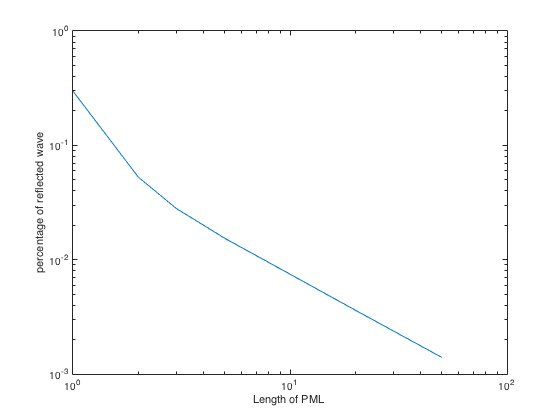
\includegraphics[scale=0.5]{images/bouncing_Lp.png}
    \caption{Percentage of reflected wave in function of $L_p$}
    \label{fig:refl_Lp}
\end{figure}
As we can observe on the figure \ref{fig:refl_Lp}, the percentage of the wave reflected at the fixed extremity of the PML and coming back in the physical medium decreases when the length of the PML increases. \\
% Length of element
Let us now focus on the length of the element $L_e$ for $20$ elements in the PML. Since the length of the PML and its coefficients of attenuation permits the complete attenuation of the incident wave, we will focus only on the reflection due to the interface.
\begin{figure}[H]
    \centering
    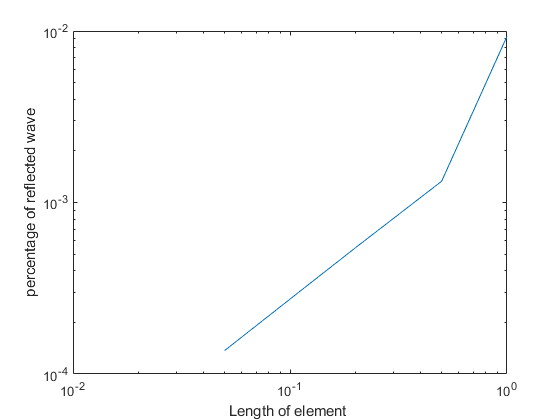
\includegraphics[scale=0.5]{images/reflected_Le.png}
    \caption{Percentage of reflected wave at the interface in function of $L_e$}
    \label{fig:refl_Le}
\end{figure}
As we can see on the figure \ref{fig:refl_Le}, the slope of the percentage of the reflected wave can be evaluated at $L_e^1$.









